\chapter{Analysis and Results}


\section{2022 vdM scan program}
\label{2022 vdM scan program}
In 2022, the main vdM scan program for the CMS experiment was conducted during LHC fills 8379 and 8381 on November 10 and 11. During fill 8381, a total of 144 bunch pairs were collided head-on , with a proton-proton collision energy $\sqrt{s}$ of 13.6 TeV. 
During this fill, various types of scan pairs with different characteristics were conducted. These scan pairs are described below. Each scan pair consisted of two scans in the transverse planes $x$ and $y$. In addition to these scans, other types of scans were also conducted, which are not included in this analysis.\\ 

The calibration program included four vdM scan pairs, vdM1,vdM2, vdM3 and vdM4, these are considered the standard vdM scans in the program, used specifically to compute $\sigma_{vis}$. In this type of scan the two beams are separated by $6\sigma_{b} \thickapprox 578\mu m$, where $\sigma_{b}$ represents the transverse bunch size. The beams are then scanned across each other in a sequence of 25 steps, each lasting 30 seconds with a step size of $0.5\sigma_{b} \thickapprox 48 \mu m$.\\

The calibration program also included two beam-imaging scan pairs, BI1 and BI2 . These scans were developed for studies on beam shapes, estimating the uncertainty caused by the not strictly valid assumption seen in previous sections that the bunch proton density function is factorizable into independent $x$ and $y$ densities, this correction is called  ($x$-$y$ nonfactorization). BI scans also are used to compute of $\sigma_{vis}$, independent of the standard vdM's scans. During the BI scans, one beam is kept fixed at its nominal head-on position, while the other beam is separated and scanned in 19 steps, each step lasts 46 seconds and covers a range from $-4.5\sigma_{b}$ to $+4.5\sigma_{b} \thickapprox 433 \mu m$.\\

Two length scale (LS) scans were conducted, one during fill 8381 and another during fill 8379. The LS scan is a special scan designed to apply a correction to the results of  $\sigma_{vis}$ obtained from the vdM scan program, this correction will be described further in this section. During this scan, the beams are separated by a constant amount of $\sqrt{2} \sigma_{b} \thickapprox 106 \mu m$, and they are moved coherently forward and backward in five steps each, all in the same transverse direction.\\

Finally two super separation periods, SS1 and SS2, were performed for the background estimation, here the two beams were sepated at a distance of $6\sigma_{b}$ during 5 minutes, at this distance the overlap of the beams is minimal and the contribution of collision is negligible.
%23:31-23:36 11:47-11:52

The scan program during fill 8381 is summarized in Figure \ref{scan_prog} where all the scans mentioned and described above are labeled.

\begin{center}
  \begin{figure}[h]	
    \centering
    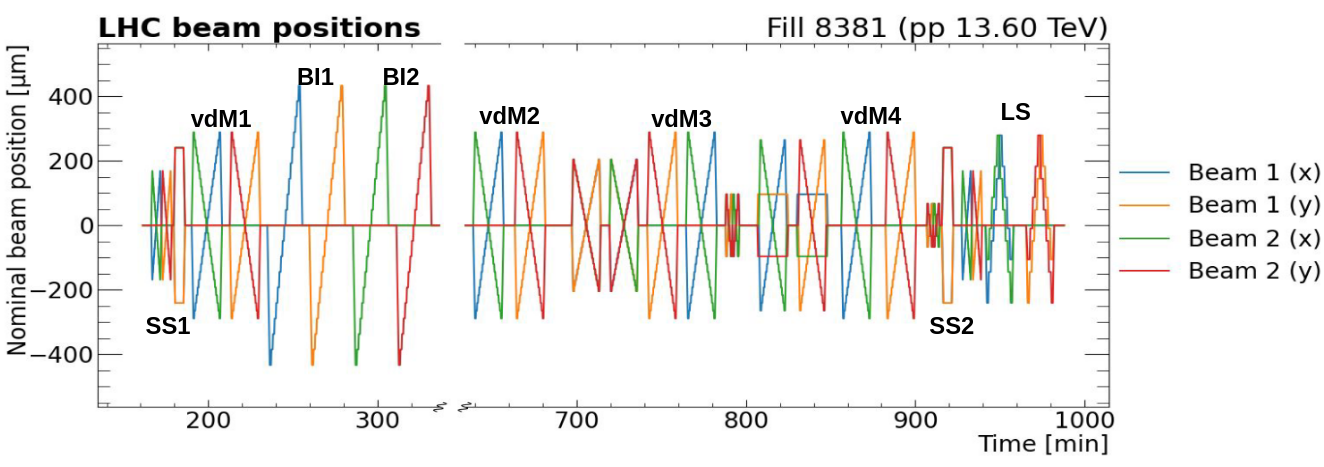
\includegraphics[scale=.35]{Chapter4/2022Scanprorgam.png}
    \caption[2022 vdM scan program]{Nominal horizontal and vertical positions of the proton beams during LHC fill 8381, showing the four standard vdM scans, two BI scans, one LS scan and the two Super Separation Periods (SS)}
    \label{scan_prog}
  \end{figure}
\end{center}

\section{Data acquisition and processing}
\label{data}
In order to achieve a high statistical precision in data for each colliding bunch pairs, the system trigger  bandwidth  limitations do not allow the use of all of bunches, because of this, CMS implemented a zero-bias triggers (defined in section \ref{Luminometers}) only on five Bunch crossing id (BCID): 282, 822, 2944, 3123, and 3302. This data is saved randomly with the highest possible rate of 27.2 kHz (5.4 kHz per BCID) using the High Level Trigger (HLT) through the CMS data acquisition (DAQ) system. Due to the weight of the events, 16 different streams are required to save the full data. Here the datasets are in the CMS RAW format, which contains information per event (bunch crossing) and the amount of charge deposited in each pixel.\\ 
During the vdM2 scan pair, the central CMS data taking was not operational, so no data was recorded for PCC, and this scan pair was skipped from the full calibration.\\

The data is then reprocessed by the CMS collaboration to enable a cluster reconstruction, resulting in the datasets (ALCARECO version) that contain a module collection and their number of clusters per event , the data here is in the CMSSW format. These datasets will be used as the starting point for our own data reprocessing and analysis.\\

The ALCARECO samples are processed using CMSSW software (written in Python and C++) to extract the clusters per module. Due to the large size of the datasets, all the datasets were sent for reprocessing through The Worldwide LHC Computing Grid (WLCG), which consists of a grid-based computer network infrastructure,designed by CERN to handle the big volume of data produced by LHC experiments. In this  process, we obtained the required cluster counts, which were saved in a dataset with a ROOT format (an open-source data analysis framework used by high energy physics) \cite{ROOT}. This format uses TTrees and TBranches, that are containers to maintain the information in a hierarchical and organized manner. 
The information is stored in one TTree that contains the information per event distributed in several TBranches, such as the number of pixel clusters, the BCID, the module identifiers, number of run, the number of lumisection (where 1 LS = 23 s), the number of luminible LN (where 1 LN is equivalent to 0.32 s) and time where that event took place (timestamp begin).\\

In order to maintain full statistical precision despite the limitations of the vdM framework (vdMFW), which was utilized for the final fit of our data, the rates were stored  each 1.32 s (NB4) time that corresponding to 4 LN, this was done making  an average  between clusters and the number of events that fall within this time span. During this process, the module veto list mentioned in the previous section is introduced and the modules detected in this list were removed. In this phase, the information is merged into a single file using a hierarchical data format (HD5) \cite{HD5} that organizes the data into tables, this final format is the required by the vdMFW. All the  process is carried out using LxBatch, a cluster of computers located within CERN.\\

Finally the HD5 file containing the rates collected during the vdM scans  is analyzed using the vdMFW, which is written in Python and uses the ROOT data analysis package through the PyRoot \cite{PyROOT} library. The vdMFW  extracts the necessary information using its analysis tools. During the process, several corrections are applied to the rates which will be described later. In the processing the vdMFW generates the final information and plots, which contain the normalized rates ($R/N_{1}N_{2}$) and beam position.  A mathematical function is then used to fit the points to extract $\Sigma_{x,y}$ and peak values to compute $\sigma_{\text{vis}}$ for all the bunches in the scan.

\section{Background estimation}
\label{bkg}
To perform accurate fitting of the data, it is necessary to take into account the following background contributions to the PCC rates. These contributions are estimated independently during the Super Separation (SS) periods discussed in the previous section. Three primary sources of beam-induced background should be considered:

\begin{itemize}

\item Beam Halo (BH): This component occurs when the secondary particles reach the experimental cavern from the LHC tunnel. The primary beam halo is  the population of beam protons characterized by offsets in the transverse coordinates, travelling in  radial amplitude around the beam axis and being captured mostly by the LHC collimation system. In every step of the multi-stage cleaning system of the LHC, more halo particles are captured but also secondary showers are created by the interaction of the beam particles with the collimator material. The largest contribution of the  beam halo to the background consist of secondary particles  that stem from the interactions of the beam halo particles at the tertiary collimators and arrive in large radius into the CMS cavern \cite{beam_halo}.

\item  Beam Gas Inelastic (BGI): This component arises from all inelastic interactions between primary beam protons and residual gas in the beam pipe. The interaction rate is largely influenced by the quality of the vacuum in the various beam line elements upstream of CMS, so the source of this contribution is distributed throughout the long straight section \cite{bkg_source}.

\item Beam Gas Elastic (BGE): The elastic beam gas contribution is made up of all the coherent and quasi-elastic, nuclear elastic, and Coulomb scattering for multi-turn beam-gas interactions around the ring.  \cite{bkg_source}.

\end{itemize}

In order to illustrate a SS period for this analisys, the Fig. \ref{ssp_wide_bx282}, correspnding to the BCID 282, displays the $<\text{PCC}>$  that is the average of pixel clusters per event in a time of 1.32s (NB4). The lower regions of the plot correspond to a time window of 5 minutes during which the beams were separated by a distance of $6\sigma_{b}$.\\

\begin{center}
\begin{figure}[h!]
\centering
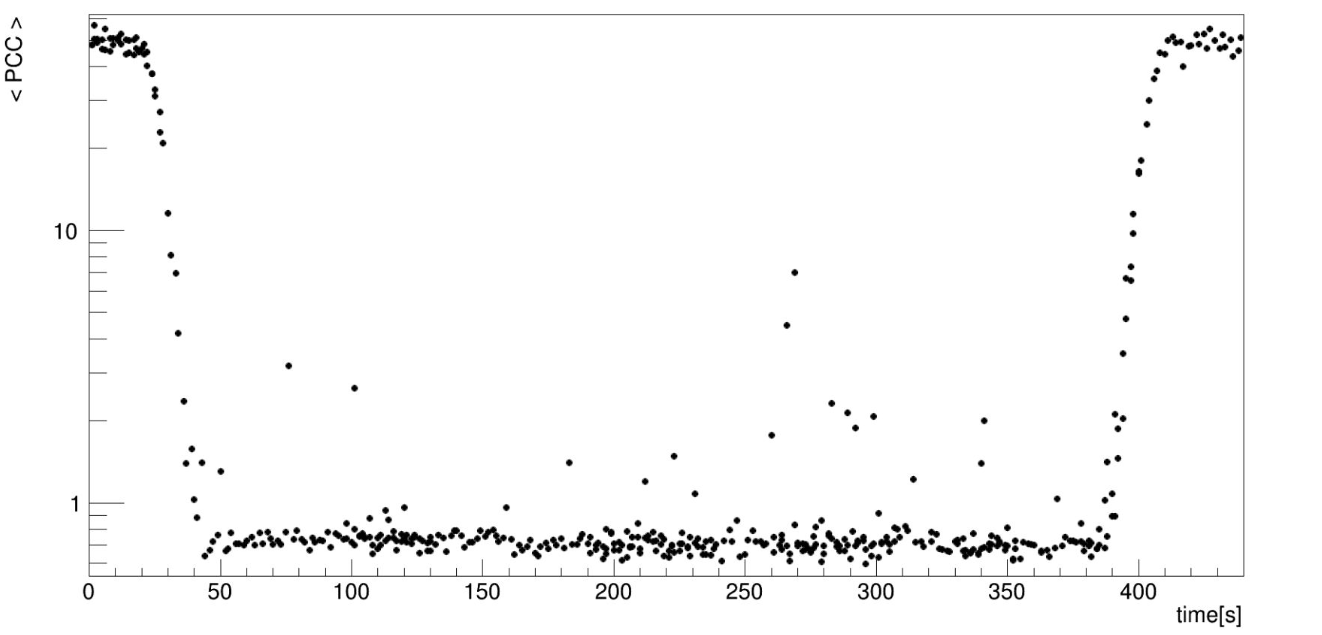
\includegraphics[width=.80\textwidth]{Chapter4/BX_282_Rates_SS1.png}
\caption[Super Separation period I for BCID 282]{Background  level for BCID 282, where $<\text{PCC}>$ is the average of pixel clusters per event in a time of 1.32s (NB4)  . The lower region correspond to the super separation period I.}
\label{ssp_wide_bx282}
\end{figure}
\end{center}

To estimate the background value, the mean value of  the  distribution of $<\text{PCC}>$ is computed. The mean and error for each super separation (SS) period are obtained taking the $y$ projection from the values showed the Fig \ref{ssp_wide_bx282}. 
To illustrate this process Fig. \ref{ss1_hist_282} displays the $<\text{PCC}>$ distribution for SS period I, specifically for BCID 282. The same plot and analysis was done  for each BCID.\\

\begin{center}
  \begin{figure}[h!]
    \centering
    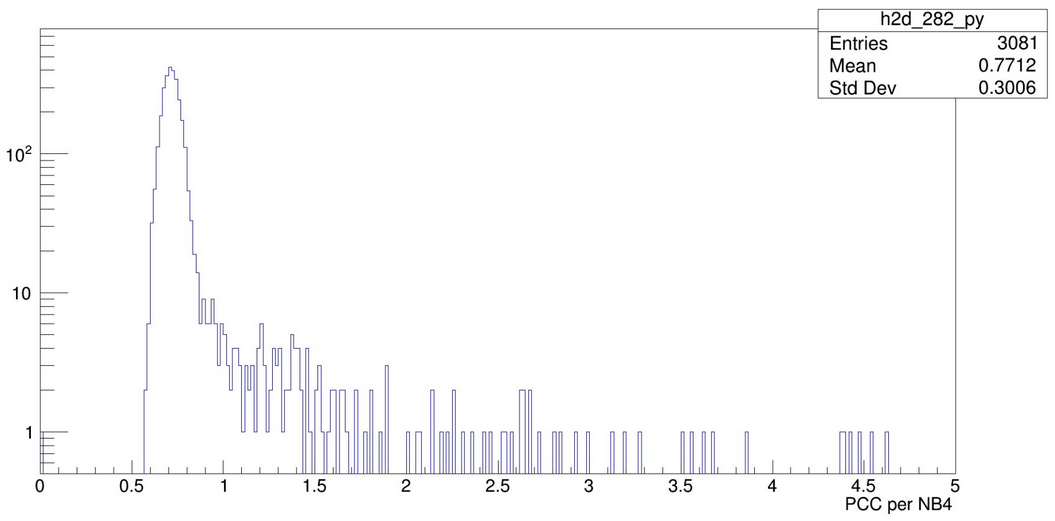
\includegraphics[scale=.26]{Chapter4/ss1_histo_bx282.png}
    \caption[$<\text{PCC}>$ profile for BCID 282 from SS period I]{profile of the $<\text{PCC}>$  for BCID 282 from SS period I.} 
    \label{ss1_hist_282}
  \end{figure}
\end{center}

\begin{table}[h!]
  \begin{center}
    \caption[Background values for the two super separation periods]{Mean and standard error on mean (SEM) for the PCC background estimated with the SS1 and SS2 data, separately for all five BCIDs and averaged.}
    \label{ss_per_bx}
    \begin{tabular}{|c | c | c | }
      \multicolumn{1}{c}{} & \multicolumn{1}{c}{\textbf{SS period I}} & \multicolumn{1}{c}{}  \\
      \hline
 \textbf{BCID}   & \textbf{Mean}   &  \textbf{SEM}\\
     \hline %\midrule[1.1pt]
      282 & 0.7734 & 0.0057\\
      \hline
      822 & 0.7756 & 0.0055\\ 
      \hline
      2944 & 0.7708 & 0.0060\\ 
      \hline
      3123 & 0.7478 & 0.0050\\ 
      \hline
      3302 & 0.7731 & 0.0052\\ 
      \hline
      \multicolumn{1}{c}{} & \multicolumn{1}{c}{} & \multicolumn{1}{c}{}\\
      \multicolumn{1}{c}{$\text{SSI}_{\text{Avg}}=$} & \multicolumn{1}{l}{$0.7680 \pm 0.0025$} & \multicolumn{1}{c}{}\\
%      \multicolumn{1}{c}{} & \multicolumn{1}{c}{} & \multicolumn{1}{c}{}
    \end{tabular}
    \hspace{0.5cm}
    \begin{tabular}{|c | c | c | }
      \multicolumn{1}{c}{} & \multicolumn{1}{c}{\textbf{SS period II}} & \multicolumn{1}{c}{ }  \\
      \hline
 \textbf{BCID}   & \textbf{Mean}   &  \textbf{SEM}\\
     \hline %\midrule[1.1pt]
      282 & 0.7207 & 0.0052\\
      \hline
      822 & 0.7247 & 0.0090\\ 
      \hline
      2944 & 0.7306 & 0.0061\\ 
      \hline
      3123 & 0.7038 & 0.0056\\ 
      \hline
      3302 & 0.7215 & 0.0056\\ 
      \hline
      \multicolumn{1}{c}{} & \multicolumn{1}{c}{} & \multicolumn{1}{c}{}\\
      \multicolumn{1}{c}{$\text{SSII}_{\text{Avg}}=$} & \multicolumn{1}{l}{$ 0.7203 \pm 0.0029$} & \multicolumn{1}{c}{}
    \end{tabular}   
  \end{center}
\end{table}

Table  \ref{ss_per_bx} shows the results for five different BCIDs, using the reprocessed PCC data for Fill 8381, where the error is calculated as $AvgErr=\sqrt{SEM_1^2 + \cdots + SEM_N}/N$. This analysis reveals notable inconsistencies in the background values obtained from the two Super Separation (SS) periods and the utilization of an average background value for all scans affected the quality of the fit. 

This circumstance prompted the implementation of a specific background value for each scan, corresponding to the time at which the scan was taken. This was achieved through an interpolation between the two background values from the SS periods. Figure \ref{interpolation} shows this procedure and the corresponding values for each scan, where the scan  times is taken from the  mean of the full scan (x and y scans) and the error asigned to these values is the mean of the two SS background errors divided by $\sqrt{2}$ assuming that there are not correlation between them. These values will be applied to each respective scan, resulting in a more consistent analysis aligned with the behavior of the background.

  \begin{figure}[!h]
  \label{interpolation}
  \begin{minipage}{1cm}
 % \label{int1}
    \begin{center}
    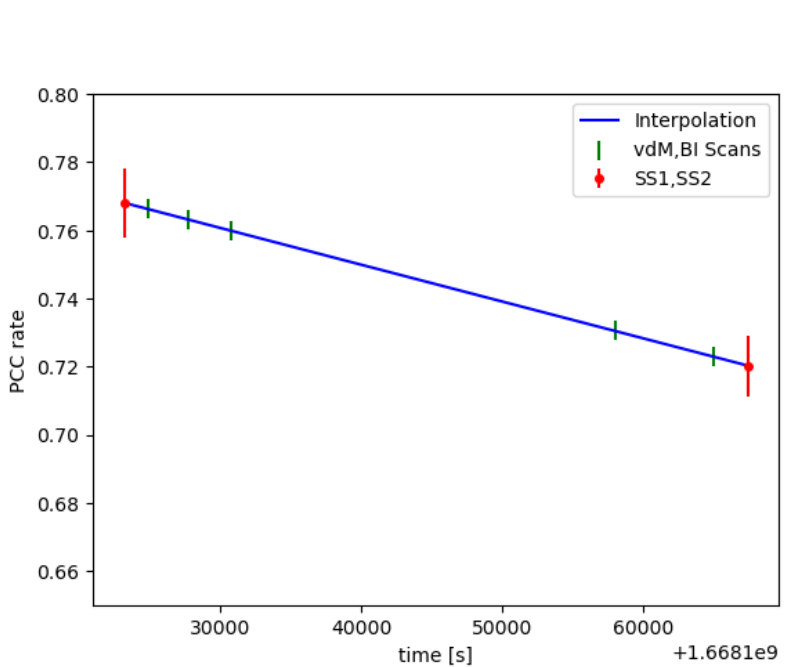
\includegraphics[scale=.3]{Chapter4/interpolation2.png}
   % \caption[Background interpolation]{ Interpolation of SS background values and time  intersection for the different scans} 
   % \label{bkg_interpolation}
    \end{center}
  \end{minipage}
  \hfill
\begin{minipage}{6cm}
%\label{int2}
\centering
    \begin{center}
%\caption[Systematic Uncertainties]{Total systematic uncertainties for the calibration.}
%\label{systematics}
\begin{tabular}{lc}
                               & \multicolumn{1}{l}{}       \\
                               & \multicolumn{1}{l}{}       \\
\textbf{Scan}            & \textbf{Background value}  \\ 
\toprule
SS1           & 0.768$\pm$0.002               \\
vdM1          & 0.766$\pm$0.007              \\
BI1          & 0.763$\pm$0.007              \\
BI2          & 0.760$\pm$0.007              \\
vdM3          & 0.730$\pm$0.007              \\
vdM           & 0.723$\pm$0.007              \\
SS2           & 0.720$\pm$0.007      
\end{tabular}
   \end{center}
  \end{minipage}
   \caption[Background interpolation]{Interpolation between the Background values ​​of the two SS periods, in red the SS values ​​are shown with their respective error, the blue line represents the interpolation and the green marks represent  the background values ​for each scan, here they follow the same order in time that has already been seen (vdM1, BI1, BI2, vdM3 and vdM4). On the right side the table is shown with the background values ​​corresponding to each of these scans}
  \label{interpolation}
\end{figure}

\section{Beam Corrections}
\label{bbcorrections}
%https://cms.cern.ch/iCMS/analysisadmin/cadilines?line=LUM-22-001
There are several systematic effects that affect the measurement of beam overlap width and therefore the extraction of $\sigma_{vis}$ from the vdM scan procedure. These effects are measured and, where applicable, corrected as described below. A systematic uncertainty is assigned to the resulting measured cross section $\sigma_{vis}$, and the following corrections are applied in the vdM Framework:
 
\begin{enumerate}

\item Ghost and Satellite. Corrects the presence of spurious charges, which affect bunch currents. Satellite charges refer to additional charges outside the actual colliding bunch, while ghost charges refer to charge not in any nominally filled bunch slot. The charges are measured by Longitudinal Density Monitors (LDMs) \cite{ghost_charge} and are corrected for with the procedure described in Ref. \cite{lumi_precise_2015_2016}.%These results in corrections of up to 0.5\% to $\sigma_{vis}$. The overall uncertaintys estimate for this  correction is 0.1\%.

\item Orbit drift. This correction accounts for potential movement of the LHC orbit during the vdM scans. Time-dependent changes of the transverse beam positions for fixed machine parameters can alter the beam separation, this correction is composed of two independent corrections: Orbit drift separation "ODS", correction that aims to correct for the orbit drift in the scanning direction and only affects beam separation and  Orbit drift rate "ODR", correction that aims to correct for the orbit drift in the direction orthogonal to the scanning direction and only affects the luminometer rate. 
%The derived correction assumes that the beam overlap has a single Gaussian shape. The correction reads the $\sigma_{vis}$ in the orthogonal direction from the previous correction. 
%Applying this correction improves the agreement between the $\sigma_{vis}$ values derived with different scan pairs and changes the average $\sigma_{vis}$ by about 0.3\%, considering the full size of the correction is as uncertainty.

\item Beam Beam corrections.  The electromagnetic interaction between the two colliding proton bunches leads to two effects in beam-separation scans:

Beam Beam deflection (BB). Corrects Beam Beam deflection that happens during bunch crossings at the collision point. Accounts for the electrical repulsion of the beams, which increases the lateral separation. The deflection is calculated and added to the nominal separation.

Dynamic Beta. The so-called dynamic $\beta^{*}$  effect, which accounts for any changes in the proton density distributions of the bunches due to the single-particle interactions. As a result, the non-linear change during separation steps in transverse bunch profiles is observed, and can described by the effective change of the $\beta^{*}$  value.
%The corrections are calculated for each proton bunch pair individually, and the combined effect of the two corrections is an increase of $\sigma_{vis}$ by 1.0\%, with an uncertainty of 0.5\%.

\item Length Scale. 
During beam separation scans, the beam positions are controlled by LHC dipole magnets and the separation is determined based on the magnet currents. To accurately calibrate the absolute scale of these "nominal" positions, dedicated length scale calibration scans are conducted. These scans involve analyzing the reconstructed pp collision vertices obtained from the CMS tracker using data from five length scale scan pairs performed in fills 8178, 8379, and 8381. The method applied here is based on the procedure described in Ref. \cite{lumi_precise_2015_2016}  

%https://indico.cern.ch/event/1244981/contributions/5230942/attachments/2581191/4452030/POG_pres.pdf
\item Residual beam positions. To investigate additional deviations of the beams, a fit model is created by combining the nominal beam positions, the orbit drift correction, and the beam-beam deflection. In order to accommodate the unknown response of the Beam Position Monitors (BPM) to the beam-beam deflection, the beam-beam deflection is scaled using a parameter that is allowed to freely vary \cite{lumi_precise_2015_2016}. Moreover, length scale factors are also included as freely floating parameters. 

In general, the residual deviations are less than 2 $\mum$. The primary source of uncertainty here is from the scale of the beam-beam deflection. Varying the scale parameter within the range of values found by the fit results in a change of $\sigma_{vis}$ of up to 1.0\%. This value is assigned as an uncertainty.\\

%\item Factorization bias. As we mentioned in section \ref{2022 vdM scan program} the vdM method assumes that the bunch proton density function is factorizable into dependent $x$ and $y$ distributions and this can lead to a biased estimate of the beam overlap area. For this, the special beam imaging scans are used. Wherein the measured vertex\footnote{A vertex is a hit recontruction that allow measure the location and the associated uncertainty, of all proton-proton interaction in each event \cite{vertex}} position distributions for $x$ and $y$ scans are fitted using aDouble Gaussian function \cite{BI_calibration,Measuring_luminosity}.

%\noindent For each fit result, the factorization bias is evaluated by comparing the luminous area ($2\pi\Sigma_{x}\Sigma_{y}$) with a simulation of a vdM scan pair that uses the fitted transverse proton bunch densities. This simulation is repeated several times to evaluate the impact of statistical fluctuations on the factorization bias. The  fit model results in a predicted factorization bias of about 0.7\% in $\sigma_{vis}$ . To account for potential additional contributions from higher order x-y correlations , twice the bias value is assigned as uncertainty.\\

%to estimate the rate at each scan step
%in the transverse bunch proton densities
\item Bunch current measurement. The number of protons per bunch are estimated from the bunch currents measured with the Fast Bunch Current Transformers \cite{LHC_bunch_populations}. A precise measurement of the total beam current is provided by the Direct Current Current Transformers (DCCTs) with a relative precision of 0.2\%, this quantity is assigned directly as systematic uncertainty \cite{DCCT_calibration_studies}. \\

\end{enumerate}

\section{Fit Model  Selection}

As we have seen in previous sections, the averaged cluster rates generated for each step of the scan need to be fitted using a mathematical function. This allows us to extract the parameters we need, such as $\Sigma_{x,y}$ and peak values for all the bunches in the scan, in order to finally compute $\sigma_{\text{vis}}$. Within vdMFW, there are several pre-defined functions that use a combination of Gaussian functions with different adjustable parameters to achieve a better fit. These functions include Double Gaussian (DG), Single Gaussian (SG), Poly Gaussians (PG), among others. All of the above functions exist in versions with an additive constant to the entire function, typically used to fit to the background levels as a separate method to the SS data.\\

For this analysis, various fit functions were tested, and the one with the best quality of fit was selected. The quality of the fit is primarily based on the convergence of the function with the points being fitted for each BCID. The convergence is assessed based on the covariance matrix, which measure the linear relationship between each pair of elements or variables. A  covariance status equal to 3 means a good convergence of the function.\\ 

The second most important parameter for measuring the quality of the fit is having a good  Chi-square $\chi^2$.  The  Chi-square goodness of fit test is a statistical hypothesis test that helps to determine whether a variable is likely to come from a specified distribution or not. This test provides a way to assess whether the data values have a good enough fit to our model, or if the model is questionable. In more general terms, this test compares observed values with expected or theoretical values according to the hypothesis. The goal is to minimize the calculation of the $\chi^2$ as defined in equation \ref{x^2}, from here is  inferred that the lower the value of $\chi^2$, the better the fit is considered to be.

\begin{equation}
\chi^{2}(\theta)=\sum_{i=1}^{N} \frac{(y_{i}-f(x_{i},\theta))^{2}}{\sigma_{i}^{2}}
\label{x^2}
\end{equation}

where the observed values $y_{1}$,···, $y_{N}$ are measured with errors $\sigma_{1}$,···,$\sigma_{N}$" at the values of $x$ given without error by $x_{1}$,..., $x_{N}$. The theoretical  value is given by the function $f(x_{i},\theta)$. The value of $\theta$ is adjusted to minimize the value of $\chi^2$ \cite{Statistical_Data_Analysis}.

After testing several mathematical fit models, the chosen model with the best fit quality and after applying all the corrections mentioned earlier, was a double Gaussian function:
%https://gitlab.cern.ch/bril/VdMFramework/-/blob/main/src/plotting/capsigma_over_time.py#L90
%\begin{equation}
%DG+Const= C+P \cdot \Biggl[ F \cdot \exp \Biggl( \frac{-(x-\bar{x})^{2}}{2 \sigma_{1}^{2} } \Biggr) + (1-F) \cdot \exp \Biggl( \frac{-(x-\bar{x})^{2}}{2 \sigma_{2}^{2} } \Biggr) \Biggr] 
%\end{equation}
\begin{equation}
f(x)= P \cdot \Biggl[ F \cdot \exp \Biggl( \frac{-(x-\bar{x})^{2}}{2(\frac{\Sigma\cdot R}{F \cdot R+1-F} )^{2} } \Biggr) + (1-F) \cdot \exp \Biggl( \frac{-(x-\bar{x})^{2}}{2 (\frac{\Sigma}{F \cdot R+1-F} )^{2} } \Biggr) \Biggr] 
\end{equation}
%[5] + [2]*([3]*exp(-(x-[4])**2/(2*([0]*[1]/([3]*[1]+1-[3]))**2))
    %    + (1-[3])*exp(-(x-[4])**2/(2*([0]/([3]*[1]+1-[3]))**2)) )
%("#Sigma","#sigma_{1}/#sigma_{2}","peak","Frac","Mean","Const")
%[0] -> [0]*[1]/([3]*[1]+1-[3])
 %[1] -> [0]/([3]*[1]+1-[3])"""
\begin{itemize}
%\item $C$ is the constant value.
\item $P$ the $peak$ rate.
\item $F$ is the fraction of the peak rate attributed to the first Gaussian in the sum.
\item $x$ is the beam position.
\item $\bar{x}$ is the mean.
\item $\Sigma$ is the overlap between the beams.
\item $R$ is the ratio between the standard deviations of the  Gaussians (first over the second).
\end{itemize}

Figure \ref{vdM1_282_XYscan} shows the fit graphs of the first vdM scan pair for BCID 282 where  all the corrections described in the previous section have been applied and where  rates are normalized by the beam currents ($N_{1}N_{2}$).

\begin{center}
\begin{figure}[h!]
\centering
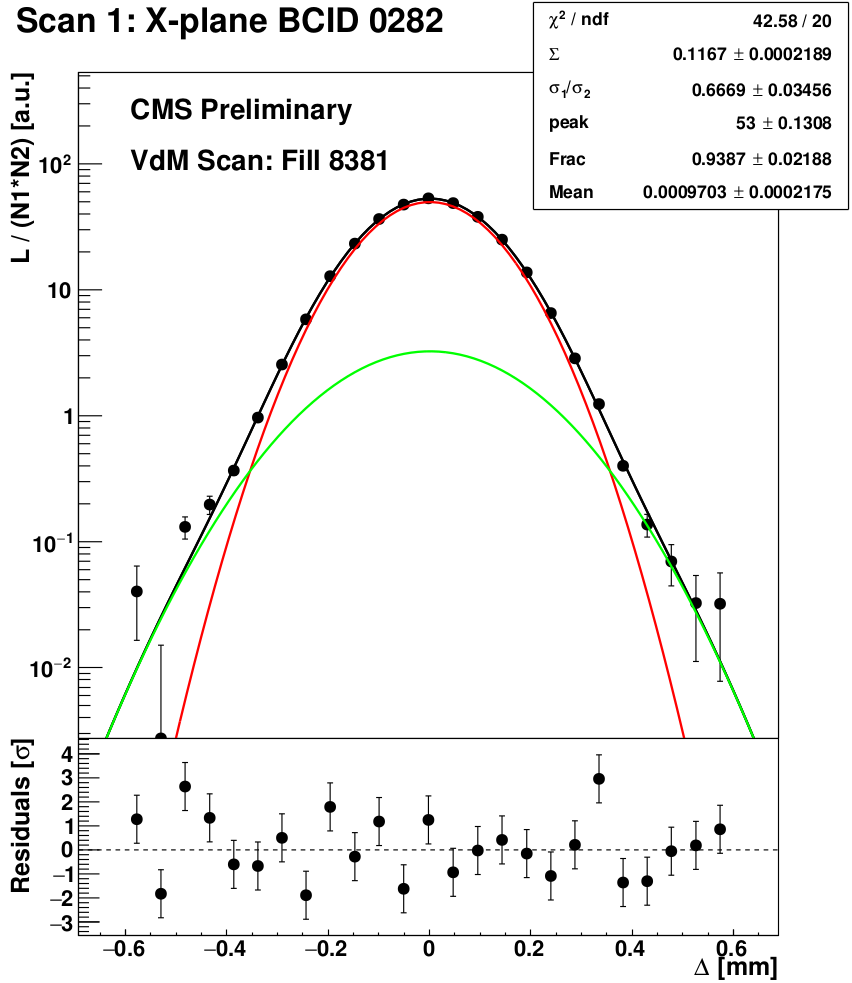
\includegraphics[width=.45\textwidth]{Chapter4/xscan.png}
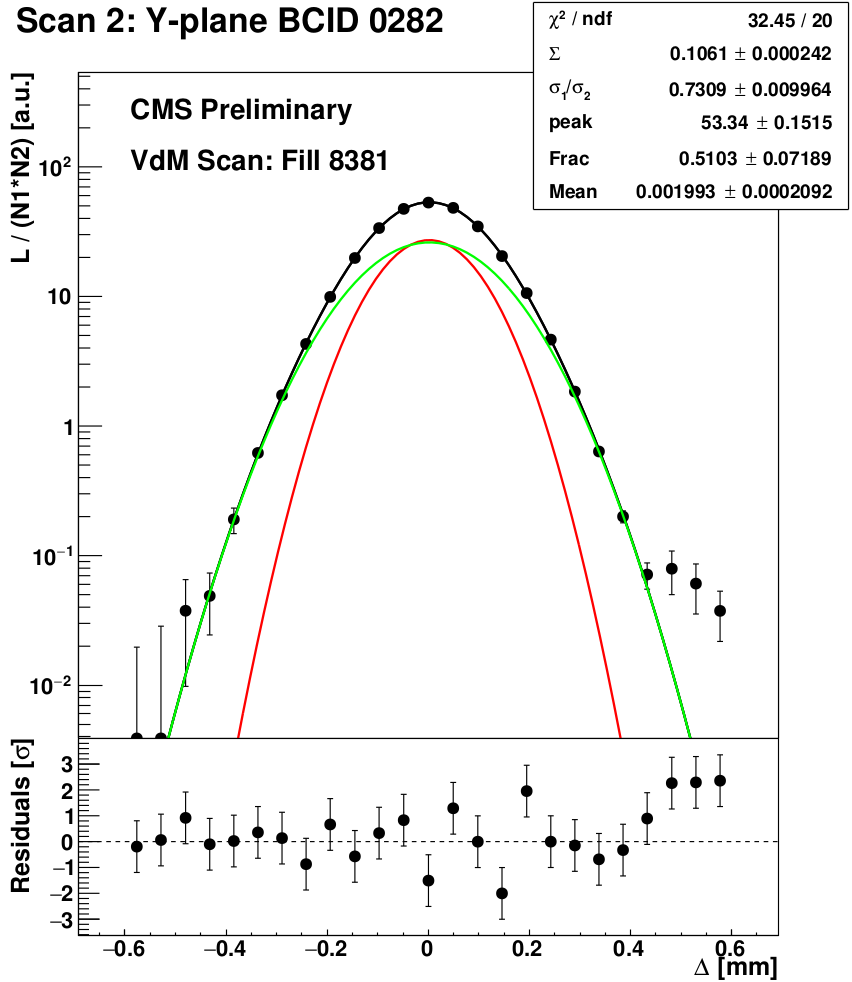
\includegraphics[width=.45\textwidth]{Chapter4/yscan.png}\\
\caption[Fit for the vdM1 BCIDs 282 (x and y directions)]{Normalized rates and the resulting fitted curves with  fit model as a function of the beam separation ($\Delta$) for BCID 282 for $x$ (left) and $y$ (right) scan for the first vdM scan.}
\label{vdM1_282_XYscan}
\end{figure}
\end{center}
For the remaining BCID's, the fits for both vdM and BI scans exhibit a very similar behavior, and in all cases, the fits have converged successfully. The evaluation of the goodness of fit is shown in Fig. \ref{chi2/ndof} where displays a plot of the $\chi^{2}/ndof$ for all the five scan pairs, which has a mean value of 1.88.

\begin{center}
  \begin{figure}[h!]
    \centering
    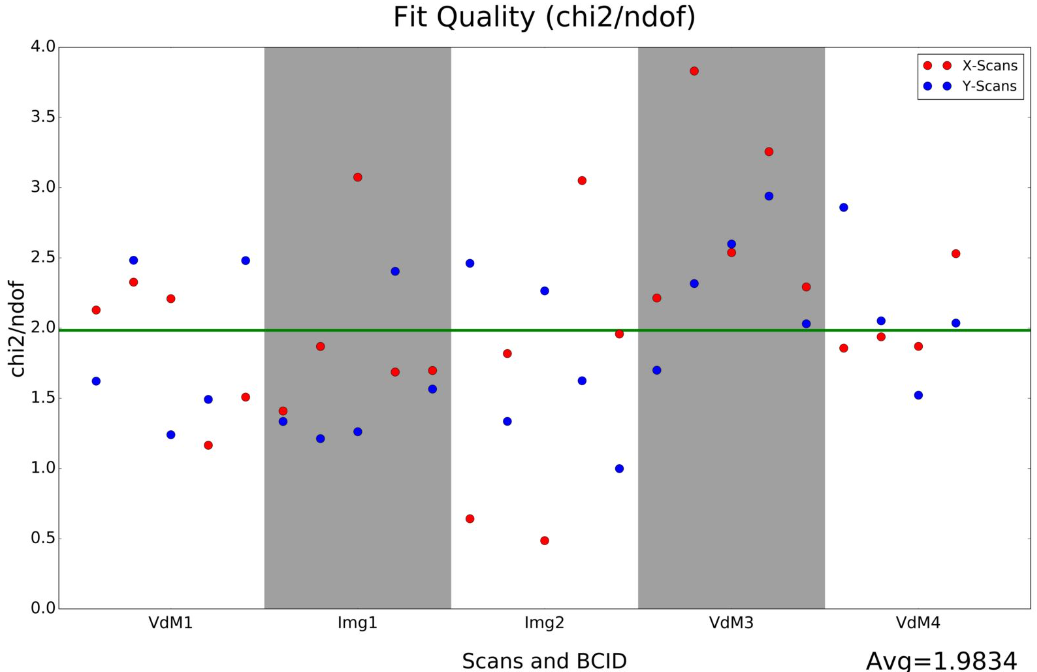
\includegraphics[scale=.30]{Chapter4/DGConst_chi2.png}
    \caption[$\chi^{2}$/ndof per BCID for all scan pairs]{ chi2/ndof for all the scan pairs.  where the red dots represent the $x$-scans, and the blue dots represent the $y$-scans. It is important to note that in each scan, the BCIDs follow the same order, which is 282, 822, 2944, 3123, and 3302.} 
    \label{chi2/ndof}
  \end{figure}
\end{center}

\section{Results}

To compute $\sigma_{vis}$, the $\Sigma_{x,y}$ and $peak_{x,y}$ values have been extracted, the behavior of these values ​​for all scans pair are shown in the  Fig. \ref{capsigma_peak} (left) for $\Sigma_{x,y}$ and Fig. \ref{capsigma_peak} (right) for the $peak_{x,y}$ values , where those belonging to the scan in $x$ are presented in red and those belonging to the scan in $y$ are shown in blue.\\

The values of $\Sigma_{x,y}$ which provide a direct measurement of the beam shape show a decrease in both the $x$ and $y$ directions during the fill time, this is due to a phenomenon called "damping", which occurs due to the interaction between the particles in the beam and the electromagnetic fields in the LHC ring, these fields exert a force on the particles, causing them to lose energy and amplitude, which causes the beam to gradually focus with time. On the other hand the values ​​for the $peak$ that are the rates on head-on normalized by the bunch currents ($R(0,0)/N_{1}N_{2}$) are then a direct consequence of the same effect, since a more focused beam means more collisions and thus a higher rate.\\

The figure also displays a discontinuity in values between the BI2 and vdM3 scans, which can be attributed to the exclusion of the vdM2 scan for the reasons mentioned in the section \ref{data} . 

\begin{center}
  \begin{figure}[h!]
    \centering
    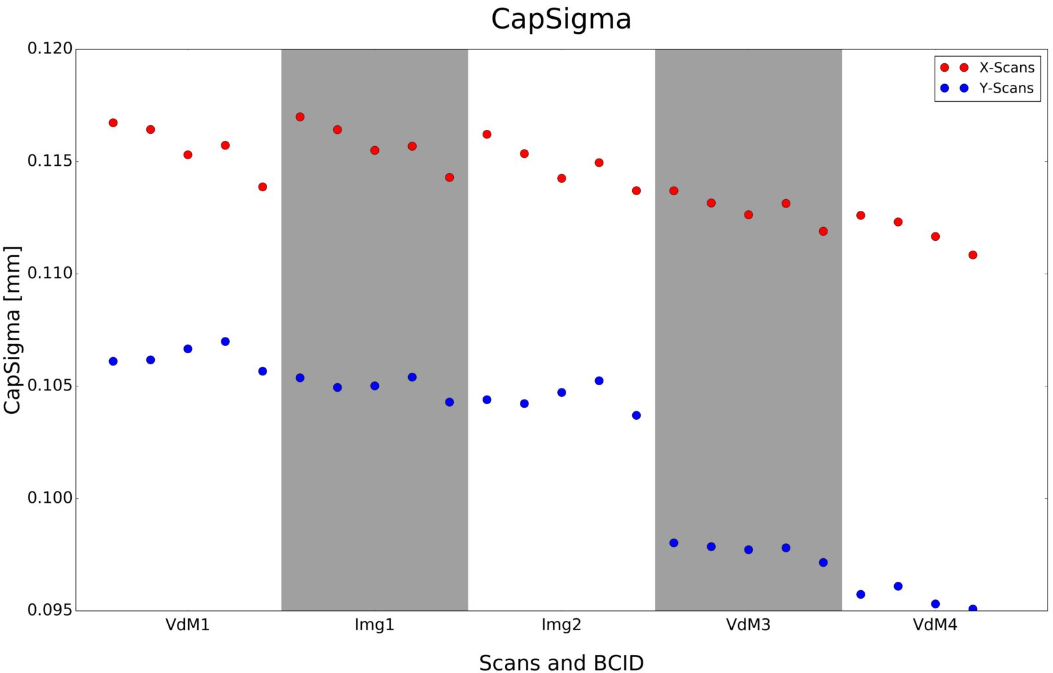
\includegraphics[width=.49\textwidth]{Chapter4/DGConst_CapSigma.png}
    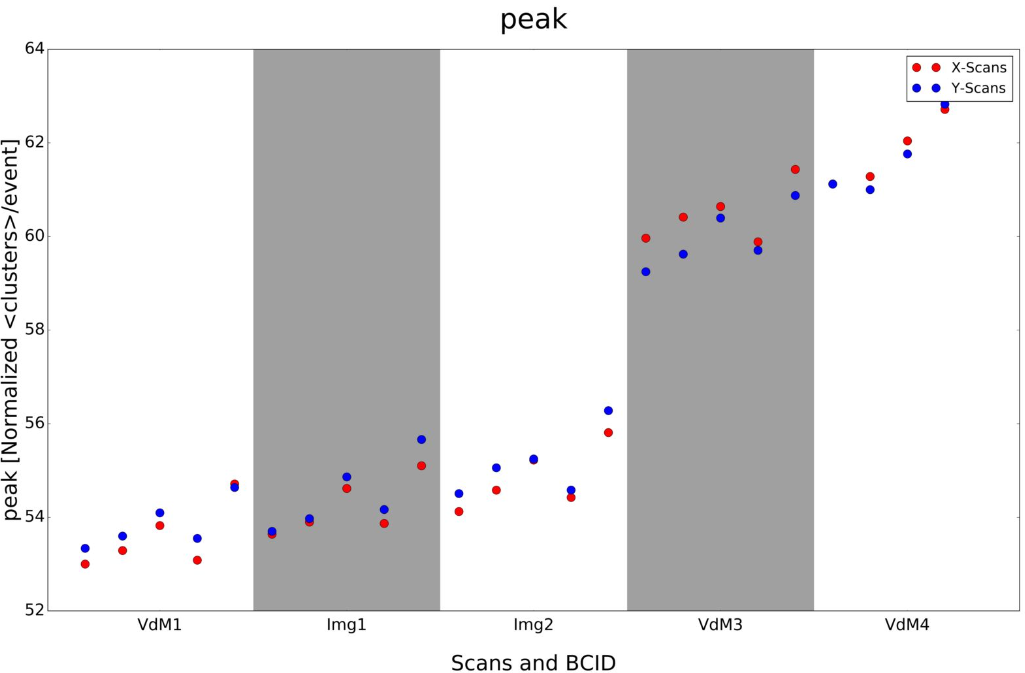
\includegraphics[width=.48\textwidth]{Chapter4/DGConst_peak.png}
    \caption[$\Sigma_{x,y}$ and peak values per BCID for all scan pairs]{$\Sigma_{x,y}$ (left) and peak values (right) extracted from the fit to compute $\sigma_{vis}$, where the red dots represent the $x$-scans, and the blue dots represent the $y$-scans, note that in each scan, the BCIDs follow the same order, which is 282, 822, 2944, 3123, and 3302.} 
    \label{capsigma_peak}
  \end{figure}
\end{center}

The $\sigma_{vis}$ for each BCID (vdM and BI scans) is then computed from the fit results $\Sigma_{x,y}$ and $peak_{x,y}$ shown above, where the final $peak$ value to use  is obtained by taking the average of the peaks in the $x$ and $y$ scans. For each bunch crossing the visible cross sections are then measured using Eq. \ref{sigmavis_eq}.

\begin{equation}
 \sigma_{vis}= \pi \Sigma_{x} \Sigma_{y}(peak_{x}+peak_{y})
 \end{equation}

Figure \ref{sigmavis_perbcid} shows the  value of $\sigma_{vis}$ per BCID for all the scans where the error on $\sigma_{vis}$ is assigned as: 

\begin{equation}
\sigma_{vis\text{Err}}= 2 \pi \sqrt{ (\Sigma_{y} \cdot P \cdot \Sigma_{x\text{Err}})^{2} + (\Sigma_{x} \cdot P \cdot \Sigma_{y \text{Err}})^{2} + (\Sigma_{x} \Sigma_{y} P_{\text{Err}})^{2} }
\end{equation}

\begin{center}
  \begin{figure}[h!]
    \centering
    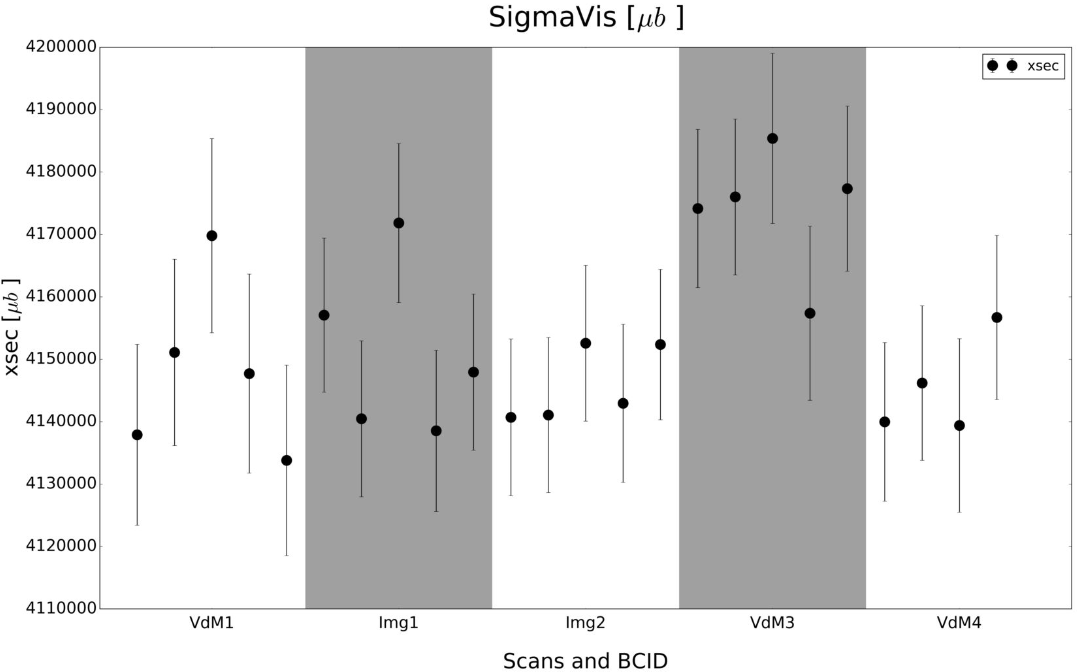
\includegraphics[scale=.30]{Chapter4/DGConst_xsec.png}
    \caption[$\sigma_{vis}$ per BCID for all scans]{ $\sigma_{vis}$ per BCID for all the scans,  in each scan, the BCIDs follow the same order, which is 282, 822, 2944, 3123, and 3302.}
    \label{sigmavis_perbcid}
  \end{figure}
\end{center}

To obtain the final value of $\sigma_{vis}$, we first perform a weighted average using 5 BCIDs for each scan as shown in Figure \ref{sigmavis_perscan} with blue dots. Subsequently, we perform another weighted average among the results of these 5 scans, this final value is represented by the red line in Figure \ref{sigmavis_perscan}. In both calculation, it is assumed that there is no correlation between the BCIDs and the scans. Therefore, the computation of the weighted average and the total error  follows Equations \ref{average} and \ref{error} respectively, where the weight is assigned as $w_{i} = 1/\sigma_{visErr}^{2}$. 


\begin{eqnarray}
\sigma_{vis}^{Avg}=\Biggl(\displaystyle\sum_{i} w_{i}\sigma_{vis}^{i} \Biggr)\Biggl( \displaystyle\sum_{i} w_{i} \Biggr)^{-1}
\label{average}
\end{eqnarray}

\begin{eqnarray}
\sigma_{vis,Err}^{Avg}=\frac{1}{\sqrt{ \displaystyle\sum_{i} w_{i}}} 
\label{error}
\end{eqnarray}

The final result obtained is:
\begin{equation}
\sigma_{vis}=4163.3 \pm 3.3 \text{ (stat)  mb}
\end{equation}

\begin{center}
  \begin{figure}[ht]
    \centering
    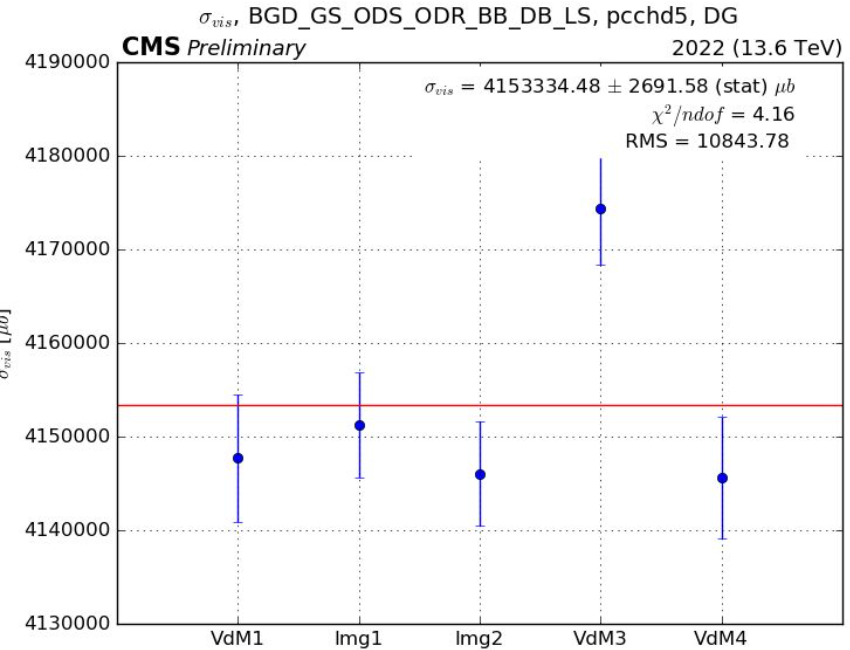
\includegraphics[scale=0.40]{Chapter4/xsec_perscan_v2.png}
    \caption[$\sigma_{vis}$ average per scan and final result]{ $\sigma_{vis}$  per scan.} 
    \label{sigmavis_perscan}
  \end{figure}
\end{center}

%As depicted in Figure \ref{sigmavis_perscan}, the scans demonstrate an RMS of $12.8 \text{ mb}$ for the $\sigma_{vis}$ values, which is larger than the statistical uncertainty. Notably, vdM1 and vdM3 exhibit the largest variations, deviating by approximately 2 standard deviations from the mean. These discrepancies can be attributed to systematic effects in the detector during the scans. Given that other luminometers display a similar trend, this could be due to a common systematic effect such as beam position or beam current $(N_{1}*N_{2})$. A study of the sources of systematic uncertainty will be performed in the future. In this work, we assign the RMS value as an estimate of the systematic uncertainty.

\section{Systematic Uncertainties}
%https://cms.cern.ch/iCMS/analysisadmin/cadilines?line=LUM-22-001
As depicted in Fig. \ref{sigmavis_perscan} and Fig. \ref{sigmavis_perbcid}, some variations in the visible cross sections from scan-to-scan and bunch-to-bunch are observed. Notably vdM3 scan exhibit the largest variation, deviating by approximately 2 standard deviations from the mean. These discrepancies are attributed to systematic effects in the detector during the scans, which, along with the uncertainty generated by the background, contribute to the final systematic error. The method for assigning an uncertainty value to these sources is described below.\\ 

\textbf{Scan-to-scan variation}: To cover the possibility of systematic differences between the scans, the standard deviation of $\sigma_{vis}$ for the five  scans is taken as uncertainty, resulting in a value of  0.26\% ($10.8 \text{ mb}$).\\

\textbf{Bunch-to-bunch variation}: The systematic of each scan is assigned as the standard deviation divided by the mean of its 5 BCIDs. Afterwards, this value is divided by the square root of the number of bunches due to the non-correlation between the bunches, as shown in table \ref{bunch-to-bunch}. The final uncertainty is assigned as the average of the systematic uncertainties from all the scans. This results in a total uncertainty of 0.1\% (3.73 mb).\\

\begin{table}[h!]
\centering
\caption[Bunch-to-Bunch Uncertinties]{Systematic uncertainties corresponding to Bunch-to-Bunch variations.}
\label{bunch-to-bunch}
\begin{tabular}{lccc}
\multicolumn{1}{c}{\textbf{Scan}} & \textbf{$\sigma_{\textbf{vis}}$ (mb)} & \begin{tabular}[c]{@{}c@{}}\textbf{Standar}\\\textbf{Deviation~(STD) }\end{tabular} & \begin{tabular}[c]{@{}c@{}}\textbf{Syst. error}\\\textbf{$\text{STD/}(\sigma_{\textbf{vis}}*\sqrt{5})$}\end{tabular}  \\ 
\toprule
vdM1                              & 4147.71               & 12.56                                                                       & 0.13                                                                              \\
BI1                              & 4151.50               & 12.22                                                                       & 0.13                                                                              \\
BI2                              & 4146.04               & 5.39                                                                       & 0.05                                                                              \\
vdM3                              & 4174.31               & 9.18                                                                        & 0.10                                                                              \\
vdM4                              & 4145.64               & 6.96                                                                      & 0.08                                                                              \\ 
\hline
\textbf{Total}                    &                          &                                                                                & \textbf{0.1}                                                                    
\end{tabular}
\end{table}
%& \begin{tabular}[c]{@{}c@{}}\textbf{$STD/(\sigma_{vis}*\sqrt{5})}\\\textbf{[\%]}\end{tabular}  \\ 
\textbf{Background}: The value of the background systematic  is assigned as the  difference between the sigma visible value obtained with a DG+Constant Fit model (4163.3 mb) and our current DG fit model with background subtraction (4153.3 mb). This revealed a difference in the $\sigma_{vis}$ of 10.0 mb, corresponding to an assigned uncertainty of 0.24\%.\\

Additionally, the beam corrections described in section \ref{bbcorrections} are taken into account, and the corresponding uncertainties have been estimated. Table \ref{systematics} displays their assigned values for the systematic error contributions. These analyses and results were obtained through independent studies conducted by the CMS team responsible for luminosity calibration.

\begin{table}[h!]
\centering
\caption[Systematic Uncertainties]{Total systematic uncertainties for the calibration.}
\label{systematics}
\begin{tabular}{lc}
                               & \multicolumn{1}{l}{}       \\
                               & \multicolumn{1}{l}{}       \\
            & \textbf{Systematic Uncertainty [\%]}  \\ 
\toprule
Length scale                   & 0.12                        \\
Orbit drift                    & 0.3                        \\
%Residual beam positions & 1.0                \\
%Factorization bias & 1.4                        \\
Beam-beam effects              & 0.5                        \\
Beam current calibration       & 0.2                        \\
Ghost and satellite            & 0.1                        \\
Scan to scan variation         & 0.26                        \\
Bunch to bunch variation       & 0.1                        \\
%Cross detector consistency     & -                          \\
Background subtraction         & 0.24                          \\ 
\hline
\textbf{Total}                 & \textbf{0.73}               
\end{tabular}
\end{table}

Taking into account the above considerations, the total systematic uncertainty is found to be 0.73\% ($77.8 \text{ mb}$). Therefore, the final value for $\sigma_{vis}$ is determined as:

\begin{equation}
\sigma_{vis} = 4153.3 \pm 2.7 \text{(stat.)} \pm 30.3 \text{(syst.) mb}
\end{equation}
